\chapter{The  ATLAS detector}
\label{ch:atlas}

\def\figpath{figures/Undergrad thesis/}


\newcommand{\AtlasCoordFootnote}{ATLAS uses a right-handed coordinate system with its origin at the nominal interaction point
in the centre of the detector and the \(z\)-axis along the beam pipe.
The \(x\)-axis points from the interaction point to the centre of the LHC ring,
and the \(y\)-axis points upwards.
Cylindrical coordinates \((r,\phi)\) are used in the transverse plane, 
\(\phi\) being the azimuthal angle around the \(z\)-axis.
The pseudorapidity is defined in terms of the polar angle \(\theta\) as \(\eta = -\ln \tan(\theta/2)\).
Angular distance is measured in units of \(\Delta R \equiv \sqrt{(\Delta\eta)^{2} + (\Delta\phi)^{2}}\).}

%-------------------------------------------------------------------------------
\section{Overview}
%-------------------------------------------------------------------------------

%%% default ATLAS stuff

The ATLAS detector~\cite{PERF-2007-01} at the LHC covers nearly the entire solid angle around the collision point.\footnote{\AtlasCoordFootnote}
It consists of an inner tracking detector surrounded by a thin superconducting solenoid, electromagnetic and hadronic calorimeters,
and a muon spectrometer incorporating three large superconducting toroidal magnets.
The inner detector system (ID) is immersed in a \SI{2}{\tesla} axial magnetic field 
and provides charged-particle tracking in the range \(|\eta| < 2.5\).
The high-granularity silicon pixel detector covers the vertex region and typically provides four measurements per track, 
the first hit being normally in the insertable B-layer (IBL) installed before Run~2~\cite{ATLAS-TDR-2010-19,PIX-2018-001}.
It is followed by the silicon microstrip tracker (SCT) which usually provides eight measurements per track.
These silicon detectors are complemented by the transition radiation tracker (TRT),
which enables radially extended track reconstruction up to \(|\eta| = 2.0\).\footnote{Text taken from the ATLAS approved detectors text section of the repo, but I'm just including the tracker info since I use hits as my variables.} 
%%% end of default ATLAS stuff

A cutaway view of the ATLAS detector is shown in \Fig{ATLAS-detector}.  The inner detector (ID) provides charged particle tracking information closer to the interaction point.  The inner detector is immersed in a 2~T solenoidal magnetic field to bend the trajectories of charged particles and allow for momentum measurement. 
\begin{figure}[h!tbp]
\centering
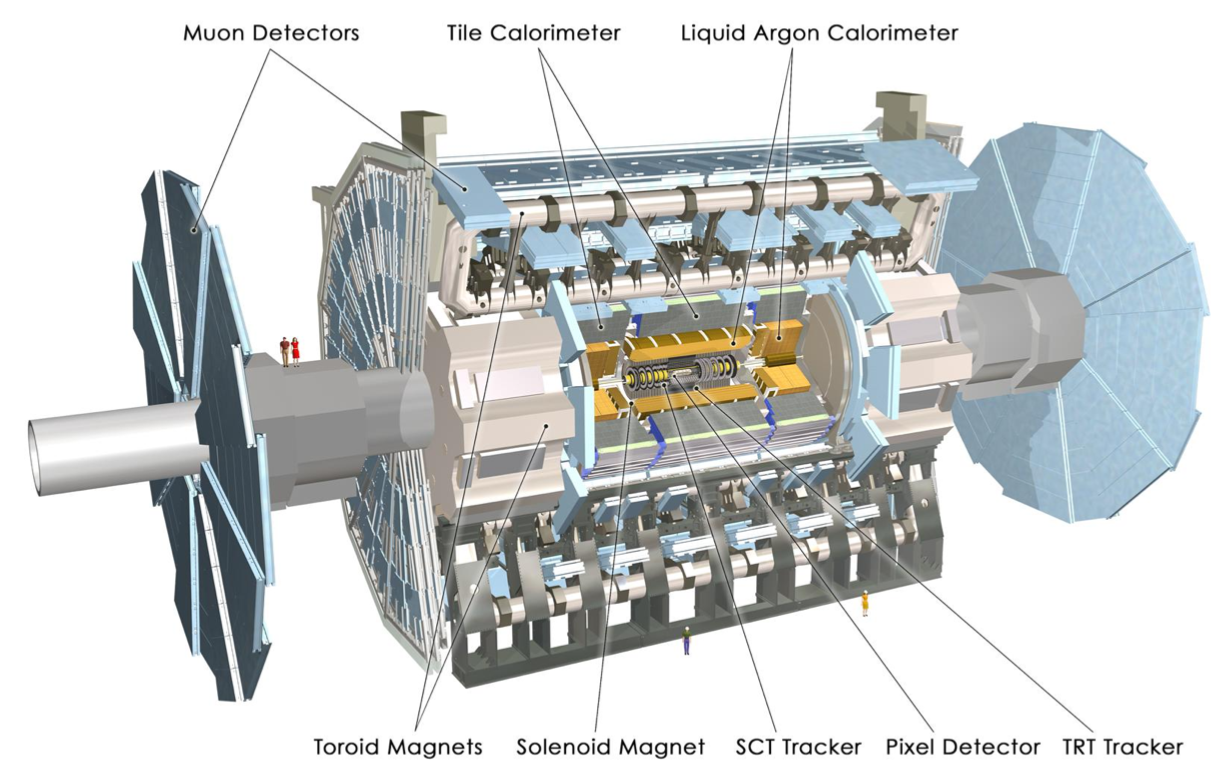
\includegraphics[width = \textwidth]{{\figpath/ATLAS_detector.png}}
\caption{Cut away of the ATLAS detector
~\cite{ATLAS_long}}
\label{ATLAS-detector}
\end{figure}
Energy measurement is made in two parts: with an electromagnetic and hadronic calorimeter.  Finally, the outermost layer of the detector is the muon spectrometer, with a 4~T toroidal magnetic field. 

\subsection{ATLAS Coordinate System}

At the ATLAS detector, the z-axis is measured along the accelerator beam pipe, the x-axis points into the center of the ring, and y-axis is defined to point vertically up by the properties of a right-handed rectilinear coordinate system.  
Then a cylindrical coordinate system is used for the ATLAS detector.
The azimuthal angle, $\phi = \arctan(\frac{y}{x})$, denotes orientation in the plane transverse to the beam, and the pseudorapidity, $\eta$, measures the polar angle inside the detector, where
%
\begin{equation}
\eta = -\ln \left( \tan \left(\frac{\theta}{2} \right) \right)
\end{equation}
%
and where $\theta \in [0,\pi]$ is the polar angle as measured from the z-axis.  The ATLAS detector is forward-backward symmetric to maximize the detector coverage since colliding protons each have the same energy.

From these detector variables, we can get components in the four-momentum using the relations %(derivation shown in Ref~\cite{eta_phi_Cartesian}).
\begin{equation}
(E,p_x, p_y, p_z) = (E,p_T \cos \phi, p_T \sin \phi,p_T \sinh \eta)
\label{momentum-conversion1}
\end{equation}
\begin{equation}
p = p_T \cosh \eta
\label{momentum-conversion2}
\end{equation}
We can also get a measurement of the momentum in the calorimeter for relativistic particles.  In the relativistic limit, the energy and momentum are the same (in natural units).  However, when the momentum is defined from a calorimeter measurement, $E_T$ is used instead of $p_T$. Equations~\eqref{momentum-conversion1} and \eqref{momentum-conversion2} still apply in this case.

\clearpage

\section{Tracker}

\subsection{Inner Detector}
\label{inner_detector}

A cutaway view of the inner detector for ATLAS is shown in \Fig{ATLAS-InnerDetector}.
\begin{figure}[h!tbp]
\centering
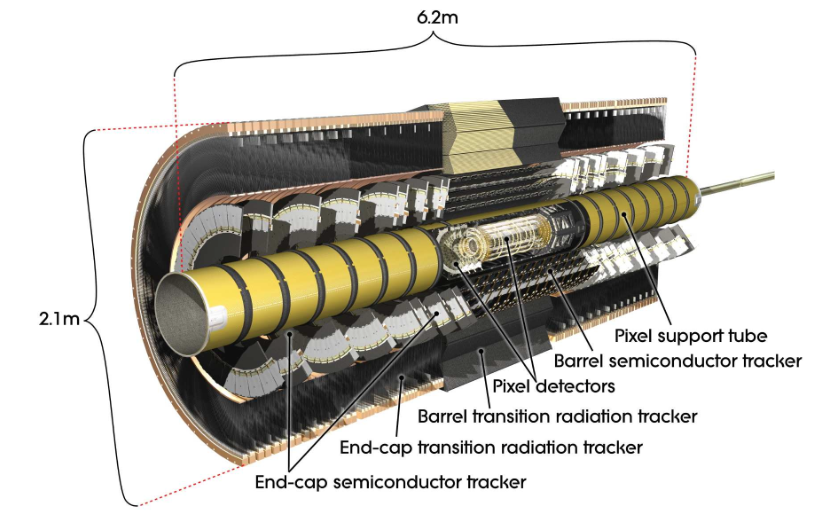
\includegraphics[scale=0.9]{\figpath/ATLAS_inner_detector.png}
\caption{Illustration of the orientation of the subsystems inside the ATLAS Inner Detector~\cite{Aad:2008Jinst}}
\label{ATLAS-InnerDetector}
\end{figure}

\begin{figure}[h!tbp]
\centering
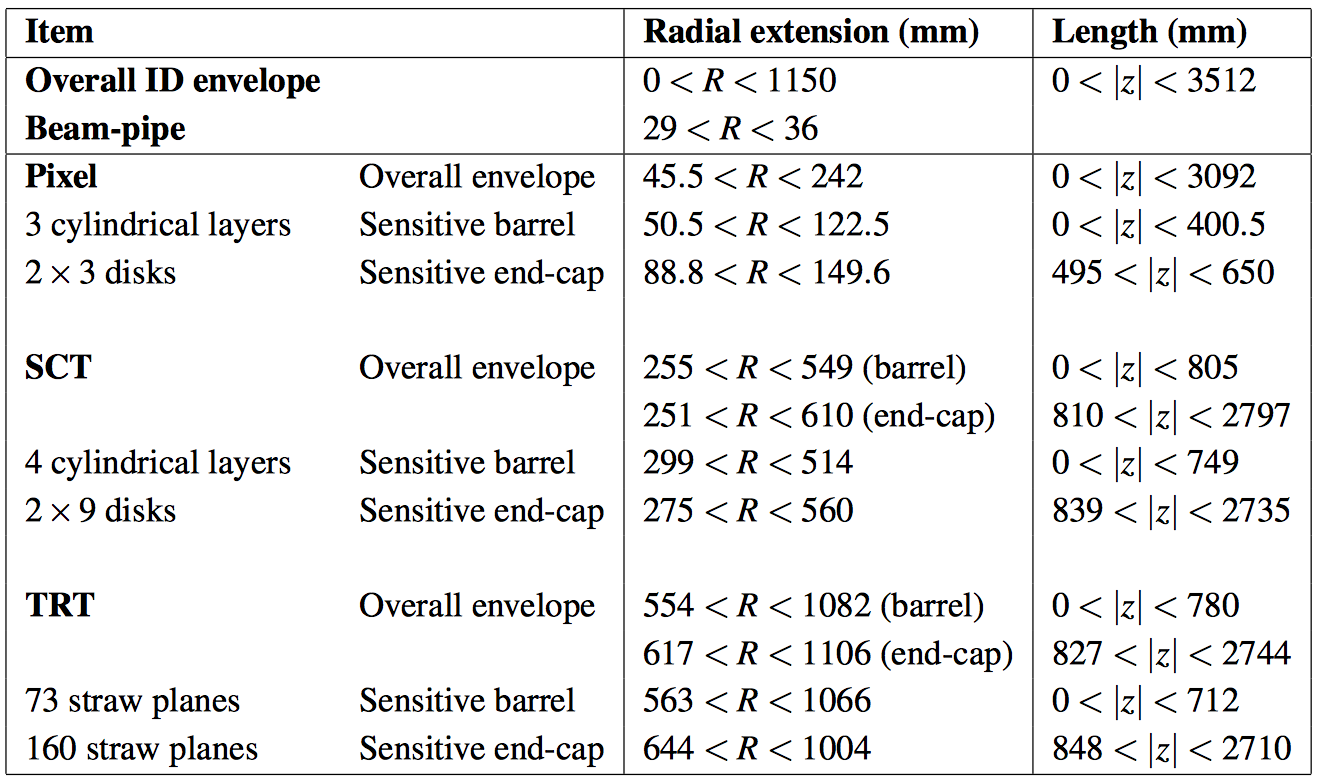
\includegraphics[width = \textwidth]{\figpath/ID_table.png}
\caption{List of the dimensions of the subsystems in the ID~\cite{ATLAS_long}.}
\label{ID-table}
\end{figure}
With approximately 1000 tracks emerging from the interaction point every 25~ns, the ID is divided into three different regions to optimize the pattern recognition and momentum measurement algorithms \cite{ATLAS_long}.  
The pixel detectors have the most precision, so this layer is closest to the interaction point. The pixel detector also has the highest cost, so the next least expensive tracking option is the silicon microstrip trackers (SCTs), at the next farthest region away from the interaction point.  Finally, the Transition Radiation Trackers (TRTs) compose the outermost region of the inner detector.
The ID uses pattern recognition to measure transverse momentum as low as 0.5~GeV, and provides electron identification for $|\eta| < 2.0$ for energies up to 150~GeV \cite{ATLAS_long}. Displaced multi-particle vertexes can be resolved by the pixel detector and help identify long-lived B-hadrons.

\begin{figure}[h!tbp]
\centering
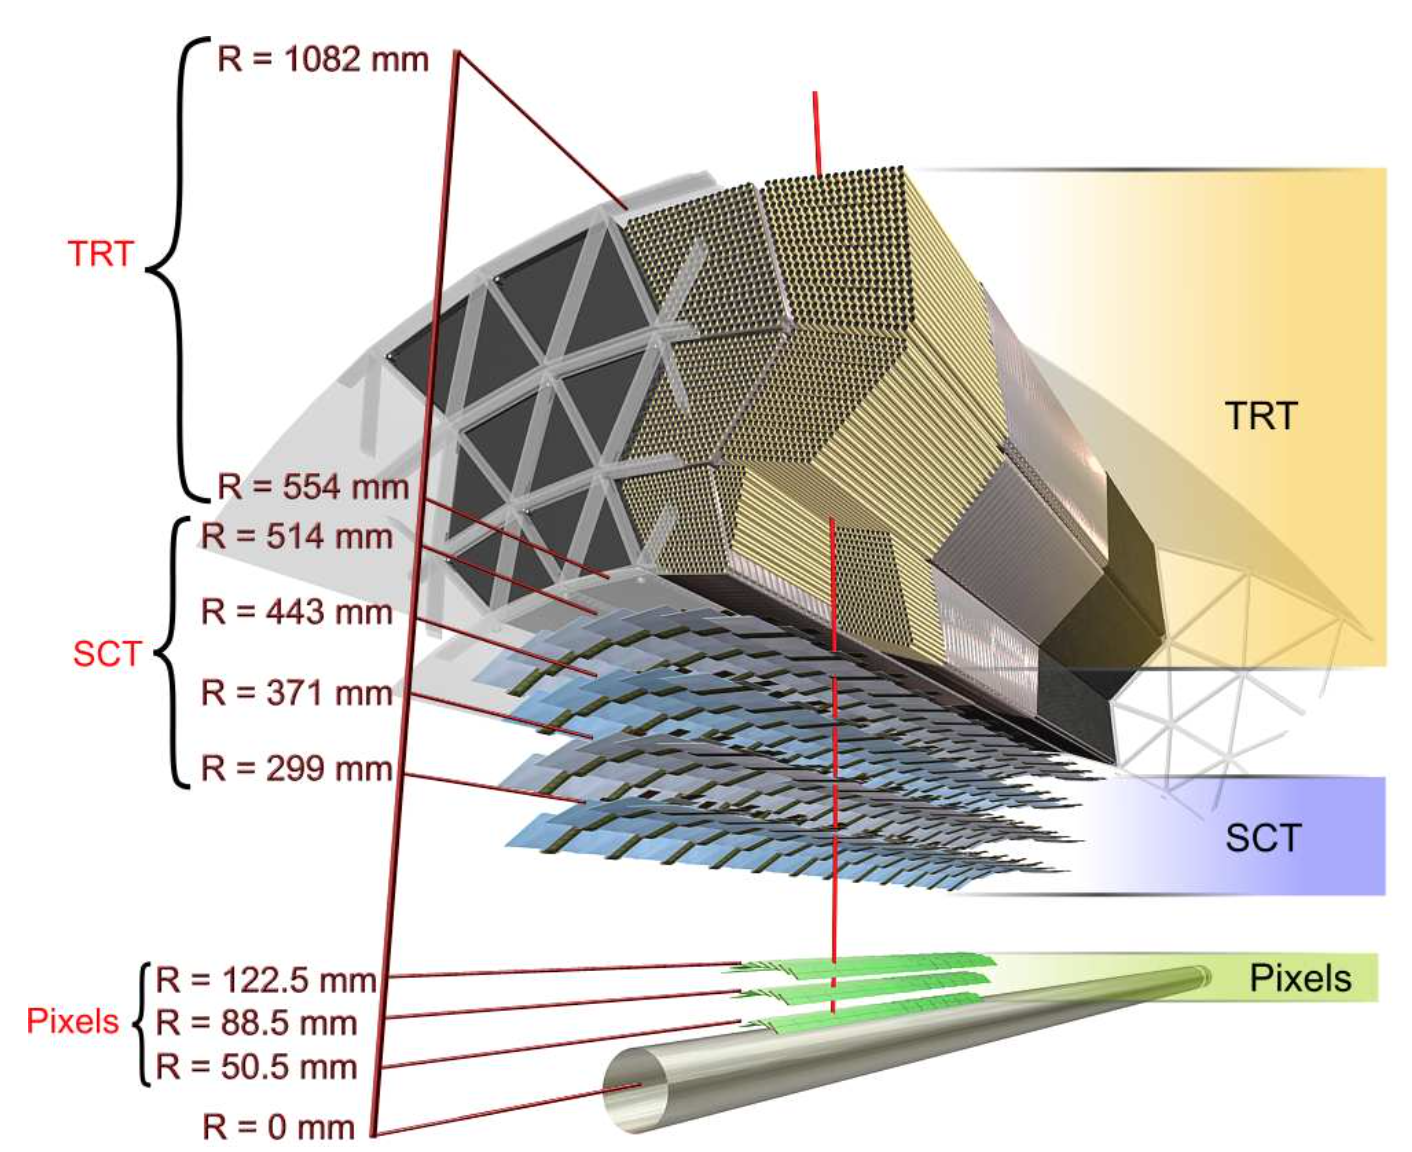
\includegraphics[width = \textwidth]{\figpath/ID_color.png}
\caption{The structural elements in the ID at $\eta = 0.3$~\cite{ATLAS_long}.}
\label{ID_color}
\end{figure}

\begin{figure}[h!tbp]
\centering
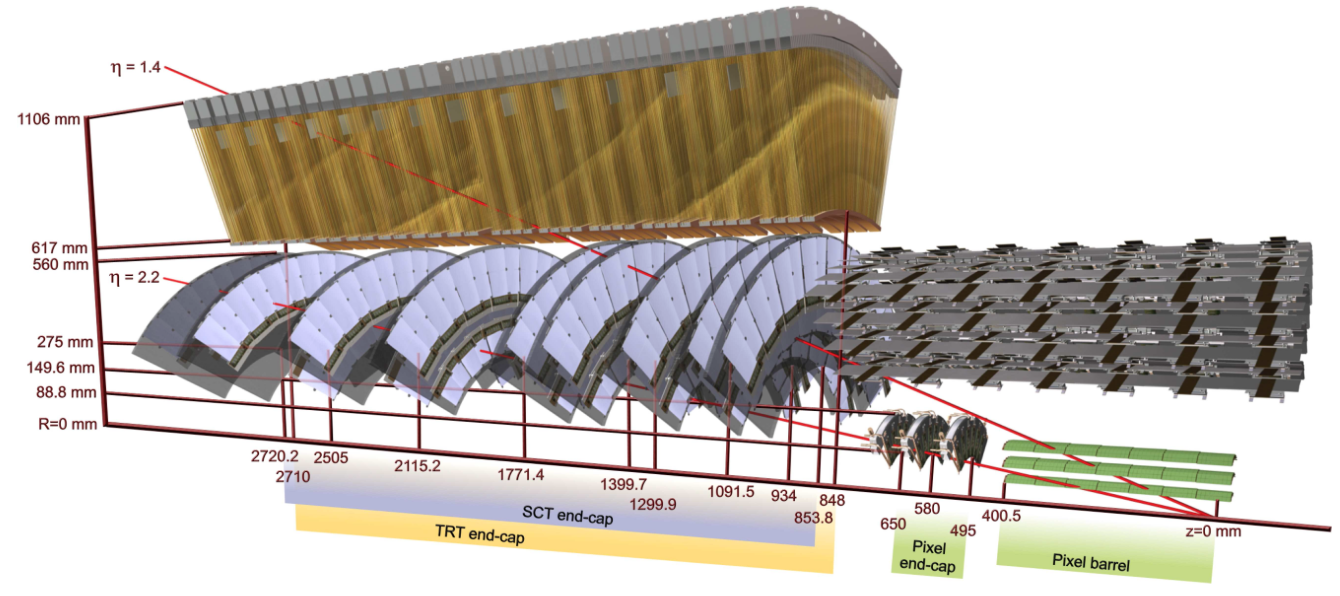
\includegraphics[width = \textwidth]{\figpath/ID_endcap.png}
\caption{The structural elements in the ID at $\eta = 1.4$~\cite{ATLAS_long}.}
\label{ID_endcap}
\end{figure}

\clearpage
\begin{wrapfigure}{r}{0.45\textwidth}
\centering
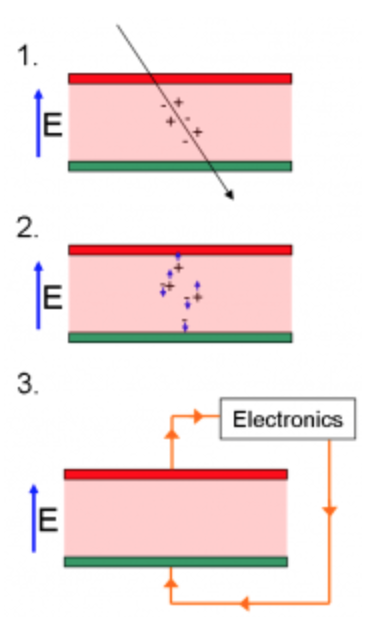
\includegraphics[width=0.4\textwidth]{\figpath/Pixel_cartoon.png}
\caption{Schematic for the general idea for how a pixel detector tracks incident particles.
~\cite{Quantum_diaries}}
\label{Pixel-cartoon}
\end{wrapfigure}

\subsubsection{Pixel Tracking System}

ATLAS is often referred to as a ``giant camera.''  
In a general sense, both a camera and the ATLAS detector provide ways to record specific events, but the parallels run deeper than their purposes, since both cameras and particle detectors can obtain information via pixels.  In a camera, an incident photon will go through a silicon diode and knock a valence electron free to generate a few electron-hole pairs.  An electric field is set up across the pixel and will then pull the electron and hole apart to the metal contacts where the charge can be read out \cite{Quantum_diaries}.  The pixel detector at ATLAS works in a similar way, except the energy of the incident particles at ATLAS is orders of magnitude larger: while a photon of visible light has an energy of a few eV, typical ``interesting'' particles at the LHC are in the MeV to TeV range.  

As a particle passes through the pixel sensor, it creates electron-hole pairs that are separated by the electric field and read out by the electronics, as shown in \Fig{Pixel-cartoon}. 

The pixel sensors in ATLAS consist of 80 million \cite{Detector_challenges} rectangular $50~\mu$m$ \times 400~\mu$m ``n$^+$-in-n'' electrodes.\footnote{The ``n'' region is n-type, or  doped with atoms that are electron donors; the ``in'' region is intrinsic, or undoped; and the ``n$^+$'' region is also n-type, but doped more heavily than other n region.}
The pixel detector's position with respect to the other components of the inner detector is shown in \Fig{ATLAS-InnerDetector}. 
Zooming in on  \Fig{ATLAS-InnerDetector}, the innermost part of the inner detector---the pixel detector---is shown in \Fig{ATLAS-PixelDetector}.  The 80 million channels are divided into four cylindrical layers combined in a volume 1442 mm in length with 430 mm radius \cite{Aad:2008Jinst}. The pixel detector has a resolution of 15 microns, and this precision is limited by the size of the electronics.

\begin{figure}[h!tbp]
\centering
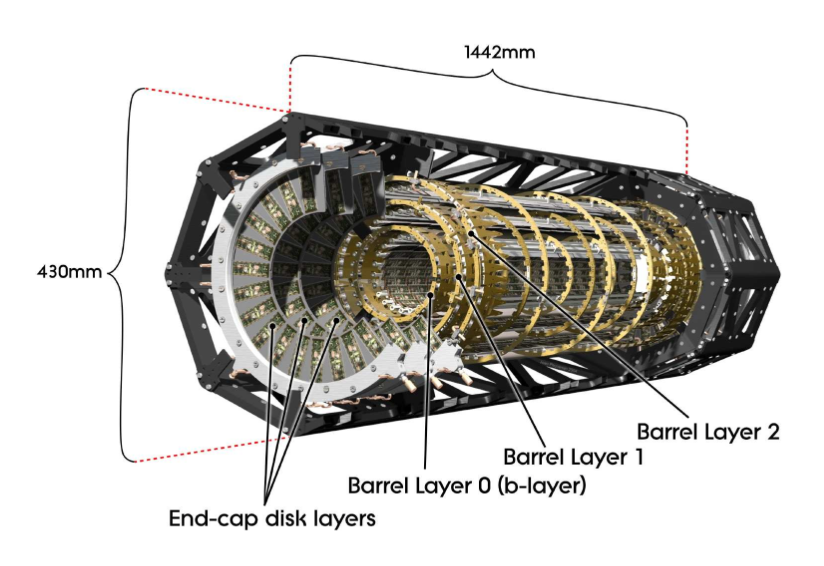
\includegraphics[scale=0.9]{\figpath/ATLAS_pixel_detector.png}
\caption{Illustration of the active region of the pixel detector with the barrel and endcap layers~\cite{Aad:2008Jinst}}
\label{ATLAS-PixelDetector}
\end{figure}

The pixel detector starts 5~cm from the center of the beam pipe to gain as much information about the central reaction as possible, and has coverage for $|\eta| < 2.5$~\cite{Detector_challenges}.
Since the pixel detector is so close to the interaction point, its electronics must be able to withstand high radiation doses of up to 500~kGy.  The p-n diodes can experience a leakage current when an electron-hole pair has enough energy to overcome the potential barrier.  
The detector minimizes the number of electron-hole pairs spontaneously generated by cooling the system at $-6^\circ$C.

\subsubsection{Silicon Microstrip Trackers}
The Silicon Microstrip Trackers (SCTs) operate with a similar principle as the pixel detectors, but have an effective operating voltage determined by the effective doping level, and their leakage current also increases linearly with radiation dose.
Initially the operating voltage was 150~V, but increased up to 250 to 350~V to compensate for the radiation dose after 10~years.
The 15912 SCT sensors each have a thickness of $285\pm15~\mu$m and a pitch of $80~\mu$m.
%(See p58 of ATLAS long for more details)

\subsubsection{Transition Radiation Tracker}
\label{trt}

The Transition Radiation Trackers (TRT) make up the outermost region of the ID, and the dimensions of the TRT are shown in \Fig{ID-table}.  ``Transition Radiation'' is the radiation emitted by a relativistic particle as it traverses an interface between two materials with different permittivities.
Each TRT is a 4~mm polyimide drift tube, created by two 35~$\mu$m multi-layer films bonded back-to-back \cite{ATLAS_long}.  
A 25~$\mu$m thick polyimide film has one side laminated with a 0.2 $\mu$m of Al with another 5-6~$\mu$m layer of graphite \cite{ATLAS_long}. 
The inside of the tube is filled with a gas composed of 70\%~Xe, 27\%~CO$_2$, and 3\%~O$_2$. 
The anode is composed of 31~$\mu$m diameter cylinder of tungsten wire positioned at the center of the drift tube, and coated with 0.5--0.7~$\mu$m of gold.
After fabrication, the tubes were cut to a 144~cm length for the barrel and 37~cm length for the end-cap region.  
The barrel straws are read out at each end of the tube, so the middle of the tube is insulated with a 6~mm glass layer which creates a 2~cm spot where the element is not sensitive to incident tracks.
The anode is grounded and connected to the front end electronics, while the cathodes are held at $-1530$V.  Minimizing mechanical sag in the straw is crucial for accounting for the error in the position measurements, so the straws are mechanically supported by carbon fibers \cite{ATLAS_long}.

\begin{figure}[h!tbp]
\centering
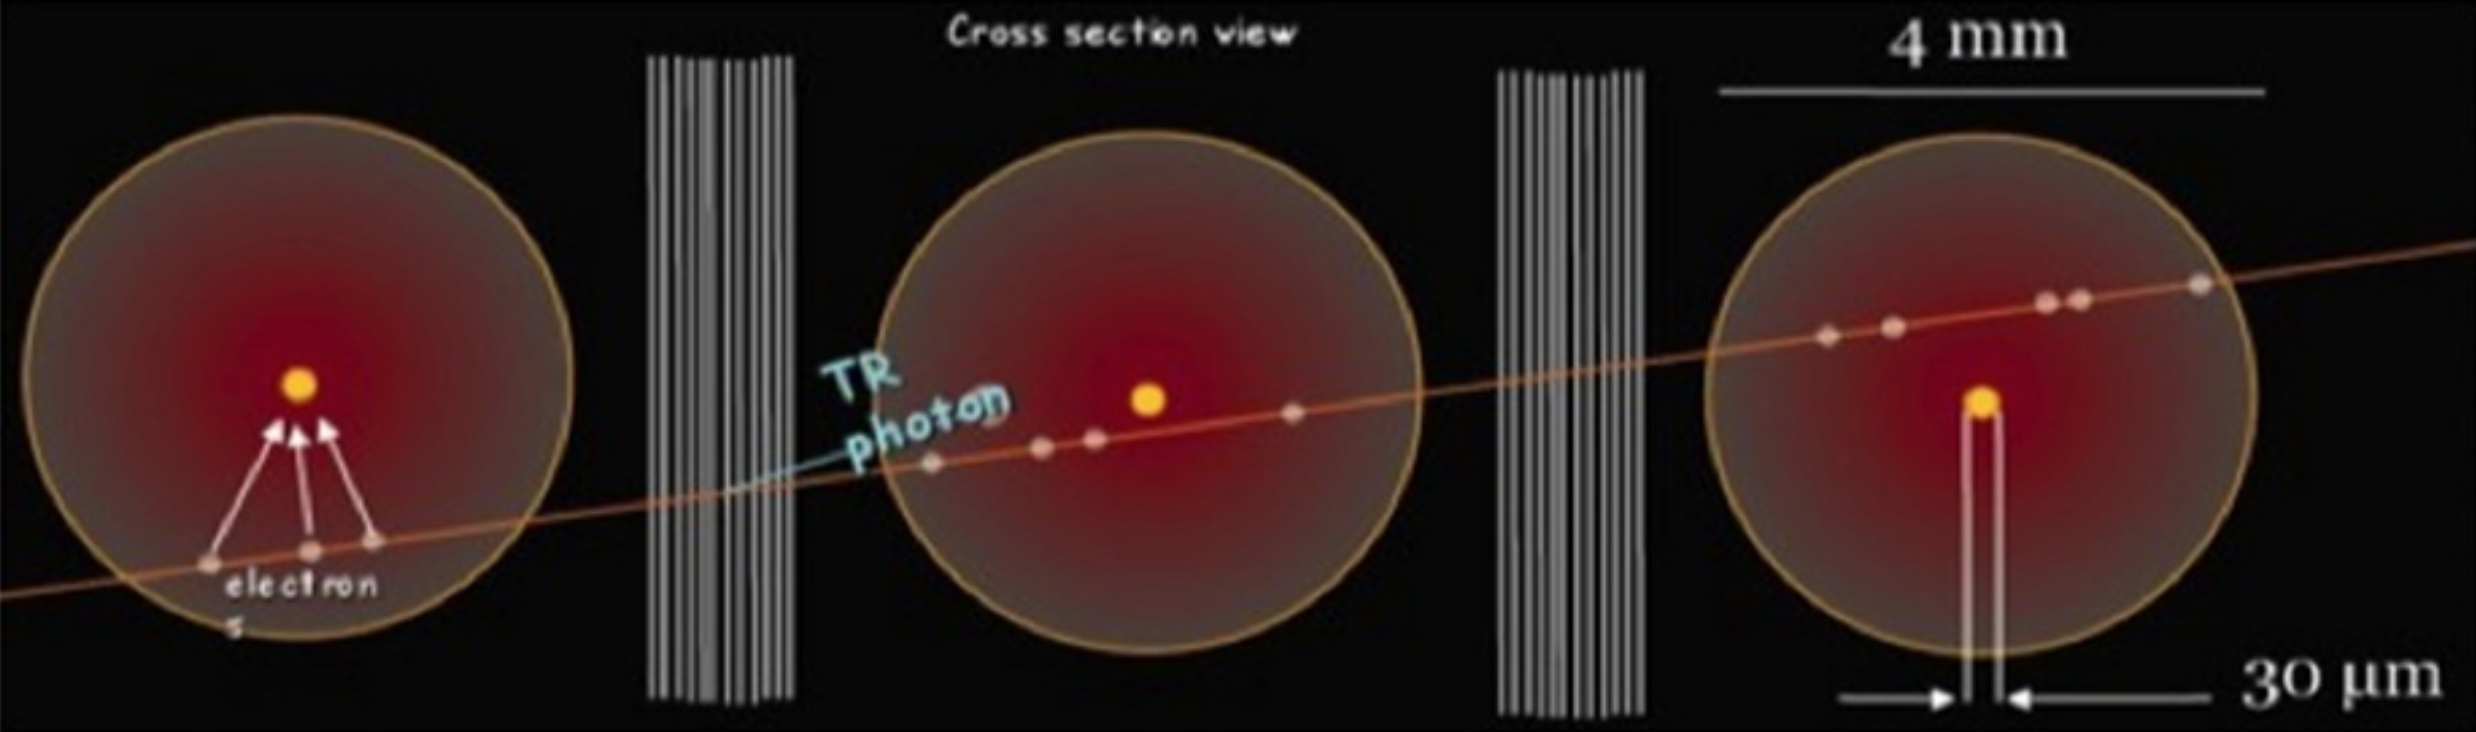
\includegraphics[width=\textwidth]{\figpath/TRT_cartoon.png}
\caption{Principle of operation for the TRT~\cite{TRT}}
\label{GEANT_sim}
\end{figure}

An incident particle traversing a straw ionizes the gas molecules to free electrons and positive ions.  The electrons accelerate through the electric field to the anode, and these electrons in turn will ionize other ions to create a gain of $2.5\times10^4$.  Since the anode is read out at both ends of the wire, this provides a drift time measurement from the difference of arrival times between the two ends of the wire.  The time resolution is approximately a nanosecond, which corresponds to a spatial resolution of about 100~microns.  

An outgoing particle will hit on average 36 of the TRT tubes; this improves the momentum measurement in the inner detector.
During its lifetime, a straw detector can track $10^{15}$ particles, and a total integrated charge of 1000~C, which corresponds to about 20~years of the LHC's operation.  
The ATLAS inner detector has 12,000 of these straws in the endcaps and 52,544 straws in the barrel, yielding a total of 351,000 read--out channels.  Although the silicon trackers need to be cooled between $-5$ to $-10^\circ$C, the TRTs operate at room temperature.

\section{Calorimeter}

\subsection{ECAL}

Calorimetry literally means ``heat measurement.'' The incident particle interacts with the material in the detector to form a shower of particles which are decelerated and absorbed in the detector material to reconstruct the original particle's energy.  
The ATLAS calorimeter is divided into two parts: the electromagnetic calorimeter (ECAL) and the hadronic calorimeter (HCAL).  The ECAL is for electromagnetic interactions and has higher precision than the HCAL which reconstructs the particles interacting by the strong force.   

\subsubsection{Sampling vs. Homogenous Calorimeters}

For an electromagnetic shower to develop, incident electrons (and positrons) will emit a photon through Bremsstrahlung approximately in through a distance characterized by the radiation length
\begin{equation}
X_0=\frac{716.4~{\text{g}} \cdot {\text{cm}}^{-2}  A}{Z(Z+1) \ln{ \frac{ 287 }{ \sqrt{Z} }}}
\label{radiation_length}
\end{equation}
where $A$ is the number of nucleons and $Z$ is the atomic number (number of protons) in the detector material~\cite{Calorimetry1}.
The units of $X_0$ means that dividing by the density gives the actual distance traveled by a particle \cite{Calorimetry2}.
Then the photons will in turn pair-produce electrons and positrons when traveling a distance of $\frac{9}{7} X_0$.  This showering phenomena will continue until the average particle energy decreases to below the critical energy, $E_c=\frac{610~{\text{MeV}}}{Z+1.24}$.
The hadronic showers are characterized by the interaction length, $\lambda = 37.8 A^{0.312} {\text{g}} \cdot {\text{cm}}^{-2}$, the average distance that an incident particle travels before undergoing a nuclear interaction.  

\begin{wrapfigure}{r}{0.5\textwidth}
\centering
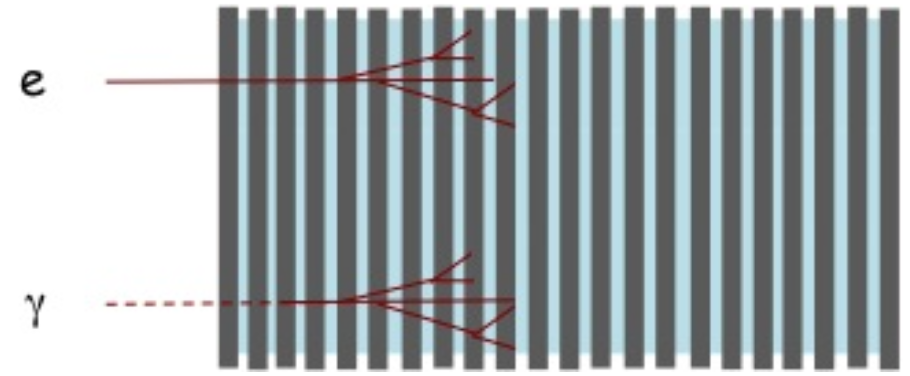
\includegraphics[width=0.45\textwidth]{\figpath/Sampling_Cal.png}
\caption{Schematic illustrating how a sampling calorimeter causes an incident particle to form a shower more quickly.
~\cite{Sampling_Cal}}
\label{sampling-schematic}
%\vspace*{-5mm}
\end{wrapfigure}

Two different calorimeter designs can be used to measure the incident particle's energy.  In a sampling calorimeter, the volume is divided into scattering and absorbing slabs, shown in \Fig{sampling-schematic}.  
The scattering slabs use a high Z material to decrease the radiation length and allow the shower to develop more quickly.  
The energy deposited in the absorbing region of the calorimeter is measured, and the total energy is the energy deposited in the absorbing region divided by a scale factor, $f_{sampling}= E_{visible} / E_{deposited}$.   A sampling calorimeter contains the shower in a smaller detector to help minimize the cost of the experiment.  
One of the downsides of this procedure is that the sampling method is not as precise because only a fraction of the energy deposited is measured, and fluctuations proportional to $\sqrt{E}$ for Poisson statistics will introduce extra errors into the measurements.

A homogenous calorimeter circumvents this problem by using the whole calorimeter as an active volume.  
A homogenous calorimeter is only useful as an ECAL since hadronic interactions require more material to ``contain,'' and it may not be monetarily feasible to construct such a large volume.  
To see this, we can look at the approximate formulas for the radiation length and interaction length, $X_0\sim \frac{A}{Z^2}$ , and $\lambda \sim A^{1/3}$. Since Z is approximately $\frac{1}{2} A$, this means  $\frac{\lambda}{X_0} \sim A^{4/3}$, a number that can be as large as 30 for high Z materials such as lead, showing that hadronic showers have a larger extent.  

\subsubsection{Liquid Argon Detector}
The ATLAS ECAL is a sampling calorimeter arranged in an accordion structure, as shown in \Fig{accordian-structure}.  The high Z material (Z = 82) lead creates the shower, while the energy is measured in liquid argon (LAr), a low Z material (Z = 18).  
As illustrated in \Fig{accordian-structure}, the folding angle decreases as the  radius (measured out from the interaction point) increases.  The folding angle varies between $90^\circ$ and $67^\circ$ to keep the LAr sampling region width approximately constant at 2.1mm between the absorbers.

\begin{figure}[h!tbp]
\centering
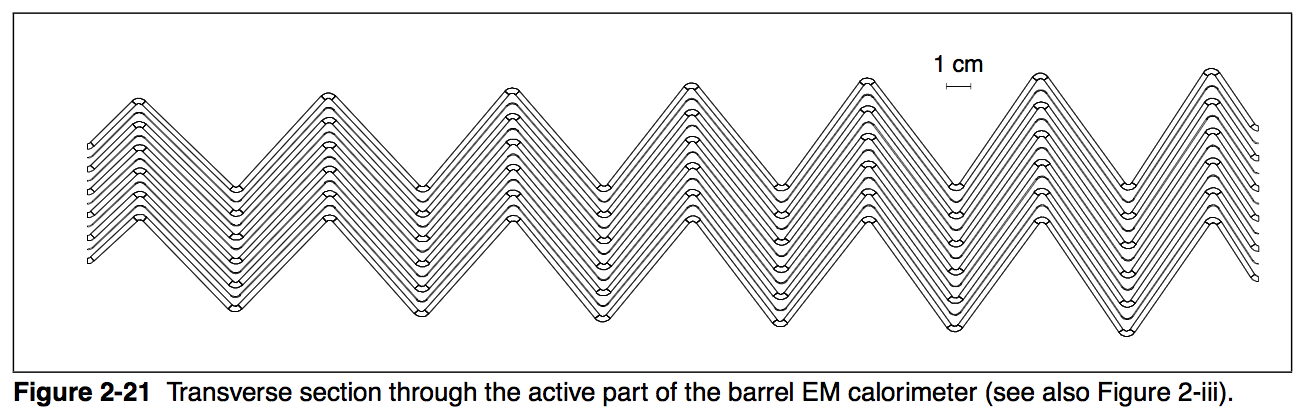
\includegraphics[width=\textwidth]{\figpath/accordian_structure.png}
\caption{Accordian sampling structure for calorimeter.
~\cite{LAr}}
\label{accordian-structure}
\end{figure}

The LAr scintillators are read out with wavelength-shifting photosensors.   
This type of a detector lends itself naturally to a tower structure with the modules forming wedges pointing back to the interaction point, shown in \Fig{Wedge-LAR-accordian}. This makes it easy for a particle's shower to be contained within a few modules or cells.  The segmentation in $\Delta \eta \times \Delta \phi$ is $0.025 \times 0.1$ in the pre-sampler region, $0.0031 \times 0.1$ in the strips, $0.25 \times 0.25$ in the main region, and $0.5 \times 0.025$ in the back region. This yields an energy resolution of 10-12\% GeV$^{-1/2}$.   

\begin{figure}[h!tbp]
\centering
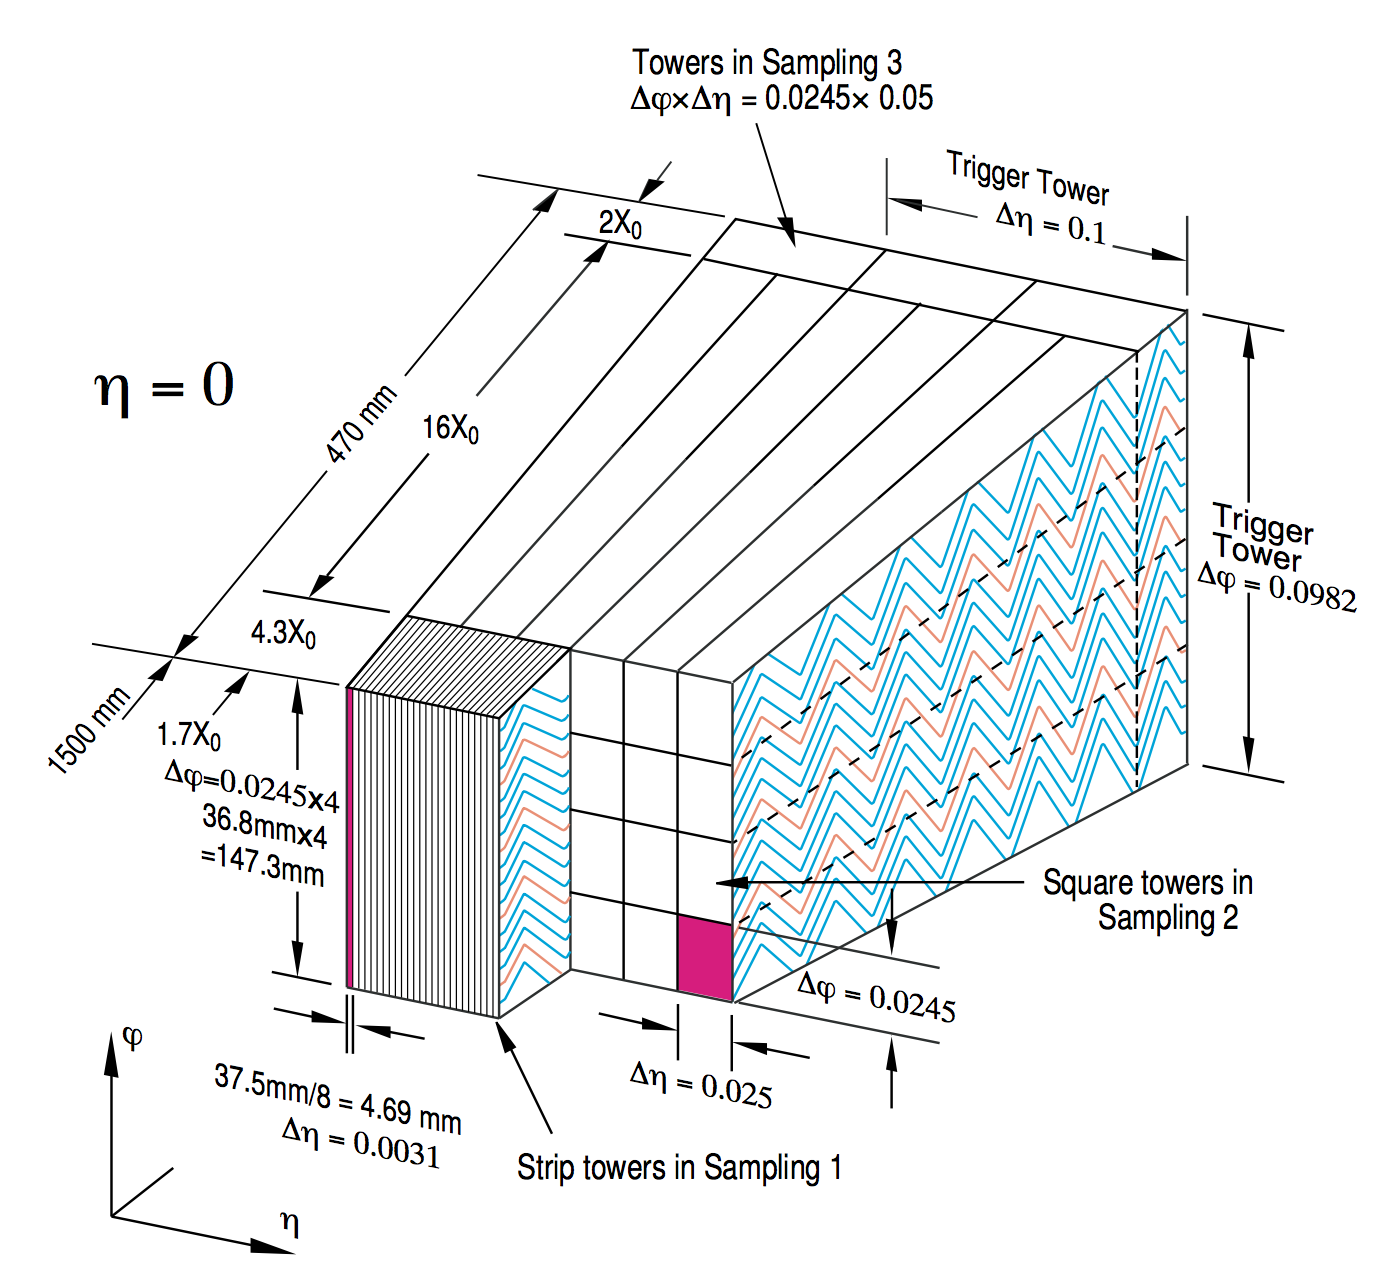
\includegraphics[scale=0.5]{\figpath/Wedge_LAR_accordian.png}
\caption{Wedge showing the accordian structure for the liquid Argon portion of the calorimeter.
~\cite{LAr}}
\label{Wedge_LAR_accordian}
\end{figure}

\subsection{HCAL}

The hadronic calorimeter (HCAL) is the layer just outside of the ECAL, and measures the 
energy of hadrons that traverse the ECAL without stopping, as well as minimum-ionizing particles like muons.
Although the ECAL system could be used to measure the development of the hadronic showers as well, the HCAL system's coarser granularity decreases the monetary cost in covering this larger volume.  It is divided into three parts: the tile calorimeter, the LAr hadronic end--cap calorimeter, and the LAr forward calorimeter, as shown in \Fig{calorimeter}.

\begin{figure}[h!tbp]
\centering
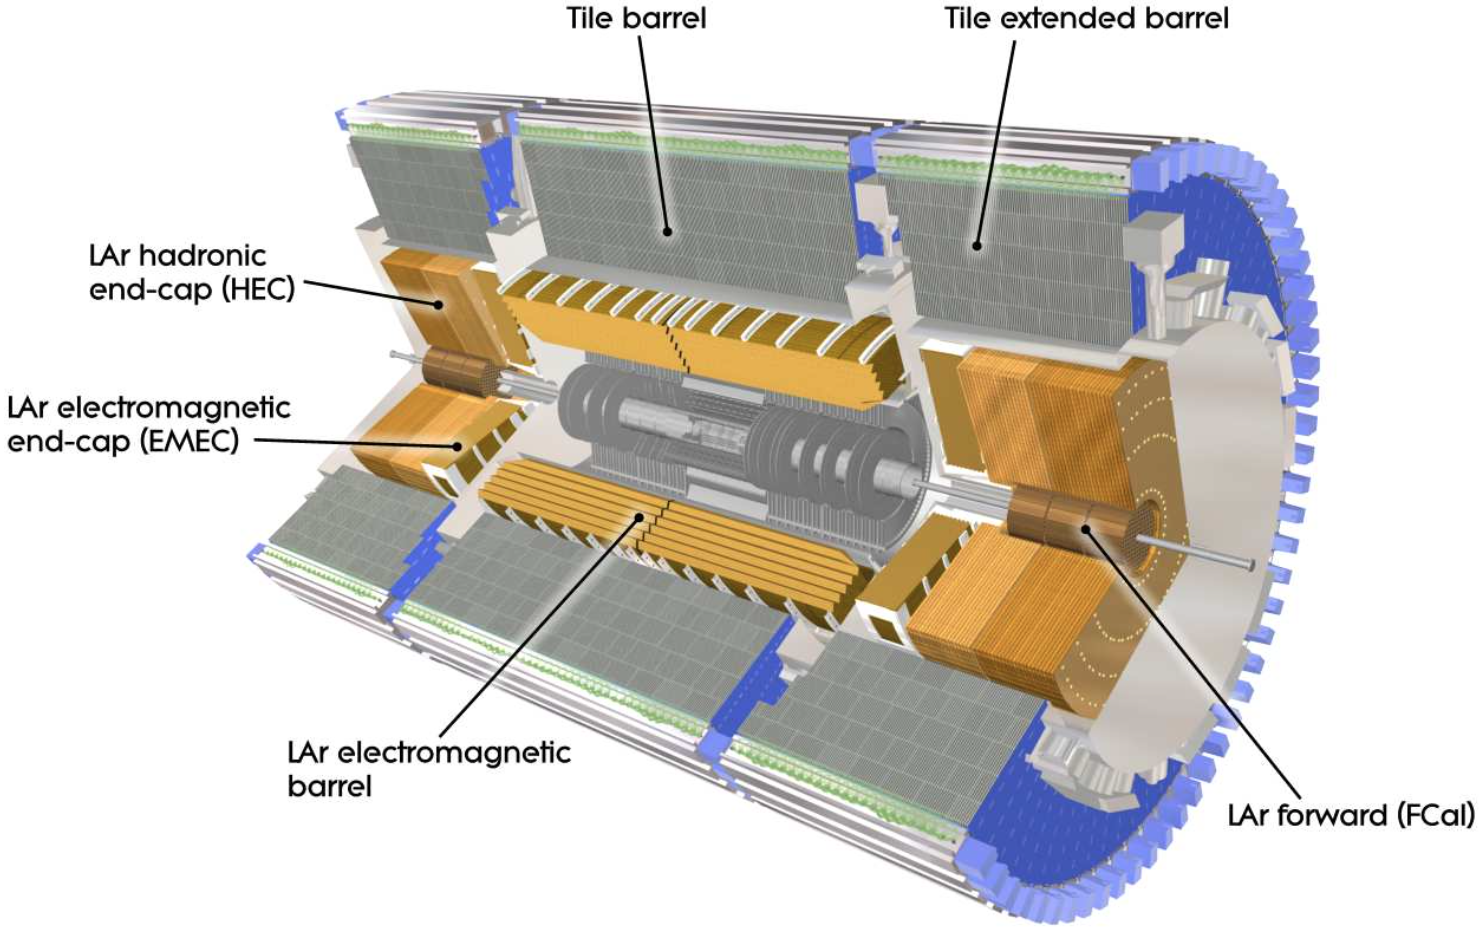
\includegraphics[width=\textwidth]{\figpath/calorimeter.png}
\caption{Calorimeter system at ATLAS~\cite{ATLAS_long}.}
\label{calorimeter}
\end{figure}

\subsubsection{Tile Calorimeter}
The tile calorimeter is just outside ECAL and has an inner radius of 2.28~m and an outer radius 4.45~m.  
The barrel covers $|\eta| < 1.0$, while the extended barrels cover $0.8 < |\eta| < 1.7$.
It is a sampling calorimeter with a steel absorber and scintillating tiles read out with wavelength shifting fibers and photomultiplier tubes. 
Azimuthally divided into 64 modules, the barrel is segmented into three regions at $1.5\lambda, 1.8\lambda$, and $4.25\lambda$, while the extended barrel has $1.5\lambda, 2.6\lambda$, and $3.3\lambda$ depth segmentation.
At $\eta = 0$, the HCAL has a 9.7$\lambda$ depth \cite{ATLAS_long}.

\subsubsection{LAr hadronic end--cap calorimeter}
The LAr hadronic end--cap calorimeter has two wheels per endcap just behind the ECAL endcap calorimeter and housed within the same LAr cryrostats.
The wheels have two depth segments, 25~mm parallel copper plates for the wheels closest to the interaction point, and 50~mm plates for the wheels farther from the interaction point.  The wheels are divided into 32 wedges, with inner and outer radii of 0.475m and 2.03m, respectively.  The copper plates are filled with LAr as the active sampling volume \cite{ATLAS_long}.

\subsubsection{LAr forward calorimeter}
The forward calorimeter covers $\eta >3.1$ and is approximately 10 interaction lengths deep.
Each side has three modules, the first of copper
 for electronic measurements, and the second two of tungsten for hadronic measurements.

\section{Muon system}

\subsection{Muon Spectrometer}

%\subsubsection{Motivation}
The tracking system determines the transverse momentum of a charged particle from its radius of curvature in a magnetic field since $R = p_T /(qB)$.  A more massive object moving at the same velocity will have a larger transverse momentum, and therefore a larger radius of curvature.  Since the muon is 200 times heavier than an electron, it can be difficult to have a tracking system that can accurately measure the momentum for relativistic muons and electrons, so the muon detection system is distinct to measure the $p_T$ for a broad range of muon energies.  

The muon detector is a gas detector like the TRT, and operates according to similar principles. 
The subsections below detail the components of the muon spectrometer, while the parameters for the coverage and number of channels for are listed in \Fig{Muon-table}.

\begin{figure}[h!tbp]
\centering
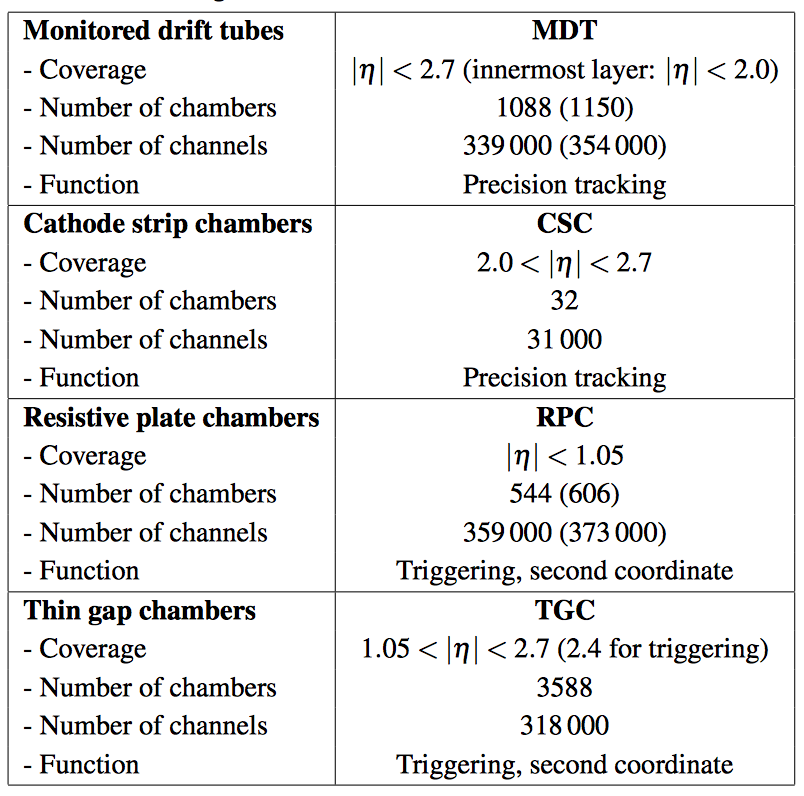
\includegraphics[width=0.75\textwidth]{\figpath/Muon_table.png}
\caption{Main parameters for the Muon Spectrometer.  The values in parentheses refer to the configuration from 2009~\cite{ATLAS_long}.}
\label{Muon-table}
\end{figure}

\subsubsection{Toroidal Magnets}

The muons are detected through the deflection of their tracks in a 4~T magnetic field.  There are three large air--core toroids, and each of these 3 toroids has 8 coils.  
The particles of interest that reach this portion of the detector are muons and neutrinos, but only the muons will be detected because the electrically neutral neutrinos are not deflected by the magnetic field.  
Backgrounds for the muon spectrometer are photons and neutrons with energies below an MeV and 100~MeV, respectively \cite{ATLAS_long}.  
The magnetic field is designed to be transverse to the muons' flight direction to minimize multiple scattering. The magnets are housed within cryostats to keep them below the critical temperature for superconductivity.  Inside these magnets are the muon chambers divided into three cylindrical chambers about the beam axis in the barrel region, while the transition and end--cap regions arranged as disks, also divided into three chambers \cite{ATLAS_long}.

\subsubsection{Monitored Drift Tubes}

The Monitored Drift Tubes (MDTs) are drift chambers that provide precision measurements. Each tube is made of aluminum with a 3~cm diameter and length between 0.9 and 6.2~m.  
The tube is filled with a 93\%~Ar,~7\%~CO$_2$ gas mixture, at a pressure of 3-bar \cite{ATLAS_long}.  It has a gain of $2\times10^4$ \cite{ATLAS_long}, similar to the TRT drift chambers (see \Section{trt}). The precision for single muon events is 100~$\mu$m, while the precision for multi-muon events is 50~$\mu$m \cite{ATLAS_long}. To control the precision, the sag of the wires is minimized by three kinematical mounts placed strategically to minimize distortion due to the support, as shown in \Fig{MDT-alignment}. There are a total of 1174 MDTs positioned in the barrel of the ATLAS detector ($|\eta| < 2$).

\begin{figure}[h!tbp]
	\centering
	\subfloat[Illustration of how an MDT works ~\cite{ATLAS_long}.]{
	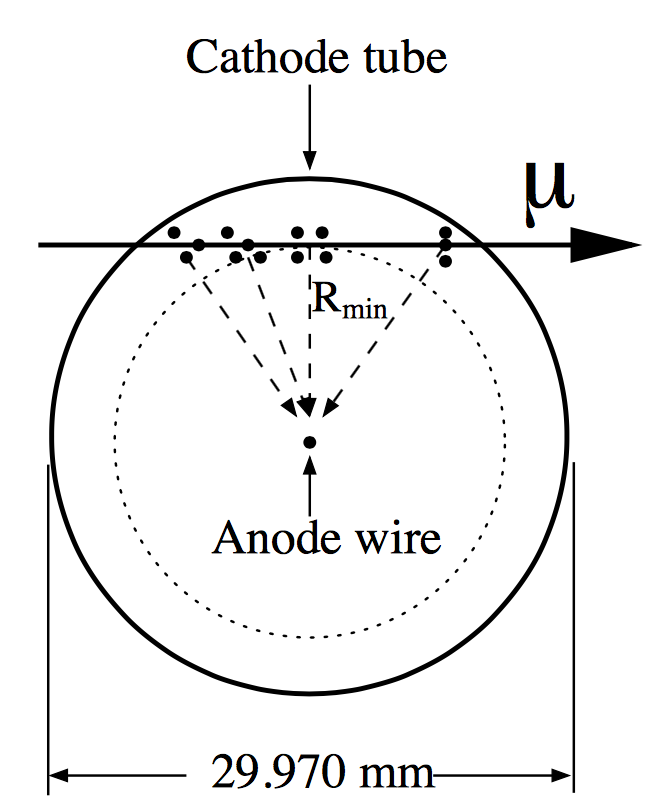
\includegraphics[width=0.25\textwidth]{\figpath/MDT_cartoon.png}
	\label{MDT_cartoon}
	}
	\subfloat[The orientation of the multi-layer MDT chamber with the support structure~\cite{ATLAS_long}.]{
	\includegraphics[[width=0.65\textwidth]{\figpath/MDT-alignment.png}
	\label{MDT_alignment}
	}
\caption{Monitored Drift Tubes: MDTs}
\end{figure}

\subsection{Cathode Strip Chambers}
\label{cdc}
For larger pseudorapidities ($2 < |\eta| < 2.7$), Cathode Strip Chambers (CSCs) are used for their higher granularity in the endcap region \cite{ATLAS_long}.  This is a multi-wire proportional chamber with strip read--out with a sense wire pitch of 2.54~mm and a read--out strip pitch of 5.08~mm resulting in a 60~$\mu$m track resolution \cite{ATLAS_long}.  

\section{Forward Detectors}
The forward detector at ATLAS covers pseudorapidities $|\eta| > 8.2$, and has three sub-systems: two to measure the luminosity and the last one for heavy--ion studies conducted when the collider accelerates with lead nuclei at $\sqrt{s}=5$~TeV.
LUCID (LUminosity measurement using Cerenkov Integrating Detector) is located $\pm 17$m from the interaction point, and is the primary online luminosity detector for ATLAS.
ALFA (Absolute Luminosity For ATLAS) is located $\pm$240~m, and uses scintillating fibers as another measure for the luminosity, with these fibers extending as a millimeter from the beam pipe.
Finally, ZDZ (Zero-Degree Calorimeter) lies $\pm 140$ and has alternating layers of quartz rods and tungsten plates for detecting neutral particles at pseudorapities $|\eta| > 8.2$ \cite{ATLAS_long}.

\section{Trigger system}


The high fluency of particles prevents the ATLAS experiment from recording every proton-proton collision.
There are three stages of triggers that discriminate which events should be written to storage.  
The Level I trigger is implemented in hardware before the information from an event even gets sent to a computing farm, and these Level I Triggering electronics need to be fast and efficient enough to pass on a manageable work load to the High Level Trigger \cite{ATLAS_long}.
The HLT records events at approximately 1000~Hz \cite{HLT}, while the beam collisions are at a rate of $4\cdot10^7$, so that the Level I needs to cut the rate by three orders of magnitude. 



\hl{Make sure I understand the magnets!!}`